\documentclass[a4paper,10pt]{article}

\usepackage[utf8]{inputenc}
\usepackage [margin = 1cm]{geometry}%permite modificar margenes
\usepackage{indentfirst}%hace que se indente tambien el primer parrafo despues de un \section
\usepackage{hyperref}%para insertar links (\href)
\usepackage{fourier}%para \danger
\usepackage{titlesec}%para el comando \titlespacing*, permite editar el espacio antes y despues de los titulos
\usepackage{graphicx}%insertar imagenes (\includegraphics)
\usepackage{xcolor}%\definecolor
\usepackage{dirtree}%mostrar items en forma de árbol 

%\titlespacing*{<command>}{<left>}{<before-sep>}{<after-sep>}
\titlespacing*{\section}{0pt}{0ex}{0ex}
\titlespacing*{\subsection}{0pt}{0ex}{0ex}

\parskip 0.15in
\setlength{\footskip}{20pt}%para que se vea bien el número de página
\definecolor{gris}{RGB}{220,220,220}

\title{Administrador de Granja - Informe}
\author{Alejandro Rivosecchi}
\date{20/08/2020}

\begin{document}

%encabezado
\begin{titlepage}
  \vspace*{2cm}
  %logo
  \begin{center}
  \large{Análisis de Lenguajes de Programación\\}
  \end{center}
  \begin{center}
  
\includegraphics[height=2cm]{fceia-logo.png}
  \end{center}
  
  \vspace{4cm}
  {\fontsize{28}{28}\selectfont\bfseries \hspace*{4cm} Trabajo Práctico Final}
  \hfill
  % Línea gris
\begin{center}
  {\color{gris}\hrule}
  \Large{\itshape Administrador de Granja}
\end{center}
    
  \vspace{13cm}
  {\large Alejandro Rivosecchi \hfill \makeatletter \@date \makeatother}
\end{titlepage}

\section{Introducción}
El programa está pensado para pequeñas o medianas granjas, kioskos o emprendimientos que tengan stock de ciertos productos y realicen ventas.

Está desarrollado y probado desde Ubuntu, pero debería ser compatible para otras distribuciones y plataformas. Utiliza \href{https://docs.haskellstack.org/en/stable/install_and_upgrade/}{stack} para manejar el proyecto.

\subsection{Secciones y uso}
\begin{itemize}
	\item Productos:

Acá figuran todos los productos disponibles a la venta con su información la cual se puede editar: nombre, proveedor, código, stock y precio. Además permite agregar y eliminar productos.
	\item Vender:

Permite realizar ventas de los productos cargados, el funcionamiento es el siguiente:

Para agregar productos a la venta ingresar la cantidad de unidades a vender y luego la tecla más.

Para retirar productos de la venta ingresar la cantidad de unidades a borrar y luego la tecla menos.

Una vez establecida la cantidad de unidades a agregar o retirar, que por defecto es una a agregar, se ingresa el código del producto y se presiona enter.

Para completar la venta se presiona enter.
	\item Ventas:

Muestra el historial de ventas ordenadas cronológicamente y permite eliminar las mismas.
\end{itemize}

\subsection{Instalación}
Una vez clonado el \href{https://github.com/murdoxix/Administrador-Granja}{repositorio} se deben instalar las siguientes dependencias:

\noindent
sudo apt-get install sqlite3\\
sudo apt-get install libsqlite3-dev\\
stack install HDBC\\
stack install HDBC-sqlite3\\
sudo apt-get install libgirepository1.0-dev libwebkit2gtk-4.0-dev libgtksourceview-3.0-dev\\
stack install gi-gtk


\danger Una de las dependencias (haskell-gi) tiene un bug con GHC 8.2.x por lo que hay que evitar dicha versión.

Se compila y ejecuta con el siguiente comando:

\noindent
stack build \&\& stack exec Administrador-Granja-exe


\section{Base de datos}
Para llevar un registro persistente de la información se utiliza una base de datos. Particularmente se utiliza SQLite3, que es una implementación de base de datos SQL en C, junto con el paquete HDBC (Haskell Database Connectivity) que permite utilizar SQLite3 desde Haskell.

La información que se aloja en la base de datos son los productos y el historial de las ventas realizadas.

El diagrama entidad/relación utilizado es el siguiente:
\begin{center}
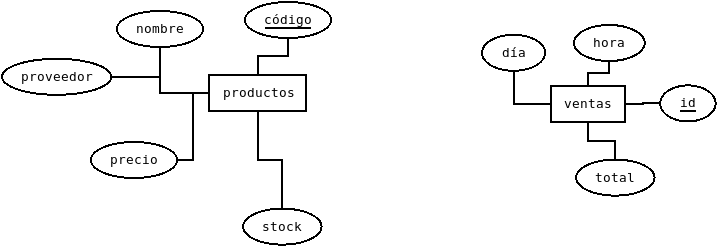
\includegraphics[scale=.5]{diagrama_entidad_relacion.png}
\end{center}

Y su pasaje a tablas el siguiente:
\begin{center}
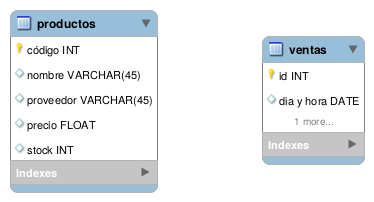
\includegraphics[scale=.5]{tablas.png}
\end{center}

\section{Interfaz gráfica}
Se utilizó GTK3 para implementar la interfaz gráfica, que es una biblioteca implementada en C para este propósito. Ademas se utilizó el paquete haskell-gi que permite utilizar GTK3 desde Haskell.

Para una pequeña y rápida introducción a GTK cito el siguiente fragmento del manual de referencia:
\begin{quotation}
GTK+ is a widget toolkit. Each user interface created by GTK+ consists of widgets. This is implemented in C using GObject, an object-oriented framework for C. Widgets are organized in a hierachy. The window widget is the main container. The user interface is then built by adding buttons, drop-down menus, input fields, and other widgets to the window. If you are creating complex user interfaces it is recommended to use GtkBuilder and its GTK-specific markup description language, instead of assembling the interface manually. You can also use a visual user interface editor, like Glade.

GTK+ is event-driven. The toolkit listens for events such as a click on a button, and passes the event to your application. 
\end{quotation}

\subsection{Glade}
Para facilitar la implementación de la interfaz gráfica se utilizó Glade, que es un programa que cumple este propósito. Permite diseñar la interfaz gráfica (crear y agregar ventanas, widgets, etc) de una manera sencilla y visual. Su output es un archivo XML que en nuestro caso es gui.glade que se utiliza para crear un GtkBuilder que nos facilita el proceso. El archivo gui.glade esta pensado para ser visto y editado justamente desde Glade.

\section{Organización de los archivos}
\dirtree{% This % is required
.1 Administrador-Granja.
.2 assets: archivos relevantes al proyecto que no son código (imágenes, informe, etc)..
.2 app: aloja el módulo Main..
.2 Base de datos: aloja la base de datos..
.2 src: aloja todo el código excepto el módulo Main..
.3 GUI: aloja los módulos relacionados con la GUI..
.4 GUI.hs: exporta la función gui que es la que inicializa la GUI..
.4 Productos.hs: módulo auxiliar para la sección Productos..
.4 Vender.hs: módulo auxiliar para la sección Vender..
.4 Ventas.hs: módulo auxiliar para la sección Ventas..
.4 Misc.hs: exporta funciones para mostrar mensajes..
.3 BibliotecaBD.hs: exporta funciones útiles para manejar la base de datos..
.3 Estructuras.hs: describe la estructura Producto utilizada..
.3 Inicializador.hs: exporta la función iniciar que crea las tablas si no están creadas..
.2 test: no lo utilizamos (creado por stack)..
}

\section{Decisiones de diseño}
Una decisión de diseño a destacar es en la diferencia del cálculo del total para las secciones Vender y Ventas. 

Para Vender decidí que cada vez que se modifica la lista de los productos por vender se calcula el total nuevamente iterando toda la lista. Esto se hizo así por la simplicidad de implementarlo y considerando que la lista de productos a vender nunca va a ser realmente grande.
\newpage
Por otro lado, en la sección Ventas, considere que calcular el total recorriendo toda la lista por cada venta agregada o removida podría ser un problema si el historial de ventas es considerable. Así que, por ejemplo, para agregar una venta se lee el total, se le suma el importe de la nueva venta y se asigna este valor como nuevo total. Al eliminar una venta se aplica el mismo procedimiento pero se le resta al total el importe de la venta eliminada.

\section{Posibles mejoras}
\begin{itemize}
	\item Asignar teclas para seleccionar cada Stack (o sección) (por ejemplo F1, F2 y F3).
	\item Mejorar el historial de ventas: que quede registrado que productos se vendieron.
	\item Mejorar la visualización de las ventas: por ejemplo poder ver las ventas por día/mes/año.
	\item Stock con cantidades reales en vez de enteras.
	\item Cuando se concreta una venta, para actualizar el stock de los productos en la store de productos la misma se recorre una a una por cada producto. Podría ser un proceso lento si hay muchos productos. Evitar esto sería una mejora.
\end{itemize}

\section{Links útiles}
\begin{itemize}
	\item \href{https://docs.haskellstack.org/en/stable/install_and_upgrade/}{stack (instalación)}
	\item \href{https://hackage.haskell.org/package/HDBC-2.4.0.3/docs/Database-HDBC.html}{HDBC (documentación)}
	\item \href{https://developer.gnome.org/gtk3/stable/}{GTK3 (manual de referencia)}
	\item \href{https://hackage.haskell.org/package/gi-gtk-3.0.33}{gi-gtk (documentación)}
	\item \href{https://glade.gnome.org/}{Glade (sitio oficial)}
\end{itemize}

\end{document}
